% ------ headers globales -------------
\documentclass[11pt, a4paper, twoside]{article}
\usepackage{header_tp2}
\includeonly{instrucciones, codigo-fuente, conclusiones, introduccion, problema1, problema2, problema3} %arreglar y agregar problema3
\begin{document}{}
% -------------------------------------
% -- Carátula --
\newpage{\pagestyle{empty}% parametros para la caratula (caratula.sty)

\materia{Algoritmos y Estructuras de Datos III}
\submateria{Entrega de TP}
\titulo{Trabajo Práctico 1}
\subtitulo{Técnicas de Diseño de Algoritmos}
\fecha{Viernes 11 de Abril de 2014}
\integrante{Barrios, Leandro E.}{404/11}{ezequiel.barrios@gmail.com}
\integrante{Benegas, Gonzalo}{958/12}{gsbenegas@gmail.com}
\integrante{Duarte, Miguel}{904/11}{miguelfeliped@gmail.com}
\integrante{Niikado, Marina}{711/07}{mariniik@yahoo.com.ar}
\grupo{Grupo \%NUMERO\_DE\_GRUPO\%}

\maketitle
\cleardoublepage}
  % -- nota:
  %       si no esta dentro de \newpage{} se rompe la numeracion y el encabezadp
  %       \cleardoublepage es para que el indice no se imprima atras de la caratula
%~ \pagestyle{empty}% parametros para la caratula (caratula.sty)

\materia{Algoritmos y Estructuras de Datos III}
\submateria{Entrega de TP}
\titulo{Trabajo Práctico 1}
\subtitulo{Técnicas de Diseño de Algoritmos}
\fecha{Viernes 11 de Abril de 2014}
\integrante{Barrios, Leandro E.}{404/11}{ezequiel.barrios@gmail.com}
\integrante{Benegas, Gonzalo}{958/12}{gsbenegas@gmail.com}
\integrante{Duarte, Miguel}{904/11}{miguelfeliped@gmail.com}
\integrante{Niikado, Marina}{711/07}{mariniik@yahoo.com.ar}
\grupo{Grupo \%NUMERO\_DE\_GRUPO\%}

\maketitle
 
\setcounter{page}{1}

%-- Índice --
\newpage{\pagestyle{empty}\tableofcontents\cleardoublepage}

%-- Dentro de TP2 redefino ciertos comandos para que se pueda compilar todo individualmente --
\begin{TP2}
%-- Introduccion --
\section{Introducción}\label{sec:introduccion}
% ------ headers globales y begin ---------------
\documentclass[11pt, a4paper, twoside]{article}
\usepackage{header_tp1}
\begin{document}{}
% -----------------------------------------------

\subsection{Objetivos}
Mediante la realización de este trabajo práctico se pretende realizar una introducción a la implementación y el análisis de las técnicas algorítmicas básicas para resolución de problemas. 

Se analizan en particular las técnicas de \textit{algoritmos golosos}, y de \textit{backtracking}.

\subsection{Pautas de trabajo}
Se brindan tres problemas, escritos en términos coloquiales, en donde para cada uno de ellos se requiere \textbf{encontrar un algoritmo} que brinde una \textbf{solución particular}, acotado por una determinada \textbf{complejidad temporal}. El algoritmo debe, además, ser \textbf{implementado} en un lenguaje de programación a elección. Los datos son proporcionados, y deben ser devueltos bajo formatos específicos de \textit{input} y de \textit{output}.

Posteriormente se deben realizar análisis teóricos y empíricos tanto de la de \textbf{correctitud} como de la \textbf{complejidad temporal} para cada una de las soluciones propuestas.

\subsection{Metodología utilizada}
Para cada ejercicio, se brinda primeramente una \textbf{descripción} del problema planteado, a partir de la cual se realiza una \textbf{abstracción} hacia un \textbf{modelo formal}, que permite tener un \textbf{entendimiento preciso} de las pautas requeridas. 

Se expone, cuando las hay, una \textbf{enumeración de las características} elementales del problema; estas son aquellas que permiten \textbf{encuadrarlo} dentro de una \textbf{familia de problemas} típicos.

Se desarrolla posteriormente un análisis del conjunto \textbf{universo de posibles soluciones} (o factibles), caracterizando matemáticamente el concepto de \textbf{solución correcta} y, en los casos en que se solicita \textbf{optimización}\footnote{Es decir, que la solución pertenezca al \textit{subconjunto de soluciones que \textbf{maximicen} o \textbf{minimicen} una determinada función}}, se definen las condiciones que dan forma ya sea a todo el subconjunto de \textbf{soluciones óptimas} que se encuadran dentro de las pretenciones del problema, o a una \textbf{solución particular} dentro del mismo (la cual denominamos \textit{mejor solución}).

Luego de caracterizar para todo conjunto posible de entradas <<\textit{cómo se compone el conjunto solución}>> correspondiente, se desarrolla un \textbf{pseudocódigo} en el que se expone <<\textit{cómo llegar a ese conjunto}>>\footnote{Una explicación coloquial, obviando detalles puramente implementativos: arquitectura, lenguaje, etc.}.

Habiendo planteado la \textbf{hipótesis de resolución} se demuestra, de manera informal o mediante inferencias matemáticas según sea necesario, que el \textbf{algoritmo propuesto} realmente permite obtener la \textbf{solución correcta}\footnote{En caso de existir más de una solución correcta, se demuestra que el algoritmo obtiene al menos una de ellas o, dicho de otro modo, para problemas de optimización, se demuestra que ninguna del resto de las soluciones correctas es mejor que la solución propuesta por nuestro algoritmo}.

Después de demostrar la \textbf{correctitud de la solución}, y su \textbf{optimalidad} en caso de existir varias soluciones correctas, se realiza un análisis teórico de la \textbf{complejidad temporal} en donde se estima el comportamiento del algoritmo en términos de tiempo. Este análisis en particular se realiza con el objetivo de obtener una \textit{cota superior asintótica}\footnote{Aunque se mencionan, sobre todo en el caso del \textit{Algoritmo de Backtracking}, algunas <<familias de entrada>> particulares bajo las cuales el algoritmo propuesto presenta un comportamiento mucho mejor al peor caso.}.

Luego de calcular la \textbf{cota de complejidad temporal}, se realiza una \textbf{verificación} empírica, junto con una \textbf{exposición gráfica} de los resultados obtenidos, mediante la combinación de técnicas básicas de medición y análisis de datos.


% -----------------------------------------------
\end{document}

\newpage
%-- Instrucciones --
\section{Instrucciones de uso}\label{sec:instrucciones}
% ------ headers globales y begin ---------------
\documentclass[11pt, a4paper, twoside]{article}
\usepackage{header_tp1}
\begin{document}{}
% -----------------------------------------------

\subsection{Herramientas utilizadas}\label{subsec:instrucciones-herramientas}

Para la realización de este trabajo se utilizaron un conjunto de herramientas, las cuales se enumeran a continuación:

\begin{itemize}
  \item \texttt{C++} como lenguaje de programación
    \begin{itemize}
      \item \texttt{gcc} como compilador de C++
    \end{itemize}
  \item \texttt{python} y \texttt{bash} para la realización de scripts
    \begin{itemize}
      \item \texttt{python} para generar casos de prueba
      \item \texttt{bash} para automatizar las mediciones
      \item \texttt{python/matplotlib} para plotear los gráficos
    \end{itemize}
  \item \LaTeX\ para la redacción de este documento
  \item Se testeó Sistemas Operativos \hfill
    \begin{itemize}
      \item \texttt{Debian GNU/Linux}
      \item \texttt{Ubuntu}
      \item \texttt{FreeBSD}, compilando a través de \texttt{gmake}
      \item \texttt{Windows}, a través de \texttt{cygwin}
    \end{itemize}
\end{itemize}

% -----------------------------------------------
\end{document}
\newpage

%-- Desarrollo --
\section{Desarrollo del TP}\label{sec:desarrollo}
  
  %-- Problema 1 --
  \subsection{Problema 1: Robanúmeros}\label{subsec:ej1}
  % ------ headers globales y begin ---------------
\documentclass[11pt, a4paper, twoside]{article}
\usepackage{header_tp1}

\begin{document}{}
% -----------------------------------------------

\subsubsection{Descripción} 

En este problema se tiene que crear un algoritmo que juegue al \textit{Robanúmeros} de forma tal 
que el jugador1 logre el mejor juego posible, y el jugador2 juegue de manera óptina durante cadu turno que le toque.
El algoritmo tiene que tener una complejidad temporal de peor caso de \bigO{n^3}, con n la cantidad de cartas
iniciales.\\
\\
Reglas del \textit{Robanúmeros}: 
\begin{itemize}
	\item Comienzo del juego: \\
	Se tiene una cantidad n ($n \in \mathbb{N}$) de cartas con valores enteros alineadas
	horizontalmente (c1, c2, ..., cn) sobre la mesa. Las cartas tienen que estar boca arriba. 
	\item Turnos: \\
	Participan 2 jugadores, cada uno va alternando un turno.(Total de turnos t: 1,..,n).  
	\item Elección de cartas: \\
	En cada turno el jugador tiene que elegir un extremo, el izquierdo (izq) o el derecho (der), de 
	la secuencia de cartas desde el que irá tomando de 1 a n de las cartas adyacentes que están en la mesa. 
	La cantidad de cartas elegidas variará según le sea conveniente al jugador, pero por lo menos tiene que tomar una 
	carta en su turno. 
	\item Fin del juego: \\
	El juego finaliza cuando no hay más cartas sobre la mesa. Se suman las cartas de cada 
	jugador (p1: Ptos. Jug1, p2: Ptos. Jug2). Gana el que obtiene el mayor puntaje.
\end{itemize}

\begin{ejemplo}\hspace{0em}

	\begin{itemize}
		\item	Cartas iniciales:
			\begin{center}
				  \begin{tabular}{|c|c|c|c|c|}
					  \hline
					   2 & -3 & -2 & 5 & 5 \\
					  \hline
				  \end{tabular}
			\end{center} 
		 
		\item   Turno1 (Jug1): Elige el extremo derecho y toma las 2 últimas cartas. 
			\begin{tabular}{|c|c|}
				  \hline
				   5 & 5 \\
				  \hline
			\end{tabular} \\

		\item	Quedan sobre la mesa: 	
			\begin{center}
				  \begin{tabular}{|c|c|c|}
					  \hline
					   2 & -3 & -2 \\
					  \hline
				  \end{tabular}
			\end{center} 	

		\item	Turno2 (Jug2): Elige el extremo izquierdo y toma 1 carta. 
			\begin{tabular}{|c|}
				  \hline
				   2\\
				  \hline
			\end{tabular} \\

		\item Quedan sobre la mesa: 	
			\begin{center}
			  \begin{tabular}{|c|c|}
				  \hline
				   -3 & -2 \\
				  \hline
			  \end{tabular}
			\end{center} 		
			
		\item Turno3 (Jug1): Elige el extremo derecho y toma 1 carta. 
			  \begin{tabular}{|c|}
				  \hline
				   -2 \\
				  \hline
			  \end{tabular} \\

		\item Quedan sobre la mesa: 	
			\begin{center}
			  \begin{tabular}{|c|}
				  \hline
				   -3 \\
				  \hline
			  \end{tabular}
			\end{center} 		

		\item Turno4 (Jug2): Sólo queda una carta, por lo que elige ésta. Es indistinto para este caso 
			  si el extremo elegido es el izquierdo o el derecho. 
			  \begin{tabular}{|c|}
				  \hline
				   -3 \\
				  \hline
			  \end{tabular} \\

		\item Finaliza el juego porque no hay más cartas. Se suman los puntajes de cada jugador.\\
			\begin{center}
			  \begin{tabular}{|c|c|}
				  \hline
				  Ptos. Jug1 & Ptos. Jug2 \\
				  \hline
				  5 + 5 + (-2) = 8 & 2 + (-3) = -1 \\
				  \hline
			  \end{tabular} \\ 
			\end{center} 	
			
		\item Formato de entrada y salida: 
			
			\begin{minipage}{0.5\textwidth}
				  \begin{tabular}{ccccccc}
					   Input: 5 & 2 & -3 & -2 & 5 & 5 \\
					   \\
					   \\
					   \\
					   \\
				  \end{tabular}
			\end{minipage} 
			\begin{minipage}{0.3\textwidth}
				  \begin{tabular}{cccc}
					  Output:  & 4   & 8  & -1 \\
							   & der & 2  & \\
							   & izq & 1  & \\
							   & der & 1  & \\
							   & izq & 1  & \\
				  \end{tabular}
			\end{minipage}
	
	\end{itemize} 	
		
\end{ejemplo}

\begin{ejemplo}\hspace{0em}

	\begin{center}
	  \begin{tabular}{|c|c|c|}
		  \hline
		   2 & -1 & 6 \\
		  \hline
	  \end{tabular} 
	\end{center} 

El Jug1 toma todas las cartas porque de esta manera obtiene el mayor puntaje. \\
Finaliza el juego en 1 turno porque no hay más cartas. Se suman los puntajes de cada jugador.\\
Este tipo de caso también se daría si todas las cartas tuvieran números positivos, sólo llegaría a jugar el Jug1.\\

	\begin{center}
	  \begin{tabular}{|c|c|}
		  \hline
		  Ptos. Jug1 & Ptos. Jug2 \\
		  \hline
		  2 + (-1) + 6 = 7 & 0 \\
		  \hline
	  \end{tabular}
	\end{center} 	
	
\end{ejemplo}



\subsubsection{Hipótesis de resolución}
Para una mayor claridad, vamos a reducir el problema a encontrar la mayor cantidad de puntos que se pueden sacar con el juego de cartas dado.\\
Sea f(i,j) = "maxima cantidad de puntos que se pueden sacar en el juego que consiste en las cartas que estaban desde la posición i \\
hasta la j en el juego de cartas original".\\
Sea suma(i,j) la suma de las cartas que estaban entre la posición i y j en el juego de cartas original.\\
Nuestro algoritmo se basa en que f(i,j) =   | valor de la carta i      si i=j\\
                                            | suma(i, j) - min(f(i', j')) para todo i' j' que representen un juego que le dejo al oponente\\
                                              usando una movida válida        sino\\
\\
\nota{habra que justificar esto?}





\subsubsection{Justificación formal de correctitud}

\subsubsection{Cota de complejidad temporal}

\subsubsection{Verificación mediante casos de prueba}

A continuación presentamos distintas instancias que sirven para verificar que el programa funciona correctamente.\\

\begin{minipage}{0.4\textwidth}
		  \begin{tabular}{cccc}
			   Input \\
			   \hline
			   n & $c_1$ & \dots & $c_n$ \\
			   \\
			   \\
			   \\
		  \end{tabular}
\end{minipage} 
\begin{minipage}{0.3\textwidth}
		  \begin{tabular}{cccc}
			  Output\\
			  \hline
			  & t   & p1  & p2 \\
			  & $e_1$ & $c_1$  & \\
			  & \vdots & \vdots & \\
			  & $e_t$  & $c_t$ & 
		  \end{tabular}
\end{minipage} \\

\begin{itemize}
	\item n: \#cartas iniciales. 
	\item $c_i$ con $1 \le i \le n$: $c_i$ valor de la carta $i$. 
	\item t: \#turnos del juego. 
	\item p1: puntaje total Jug1.
	\item p2: puntaje total Jug2.
	\item $e_i$ con $1 \le i \le t$: $e_i$ extremo elegido por el jugador en el turno i (izq o der). 
	\item $c_i$ con $1 \le i \le t$: $c_i$ \#cartas tomadas por el jugador en el turno i. 	
\end{itemize}
				
Según los valores de p1 y p2, podemos separar en 3 casos posibles: 
				
\begin{enumerate}
	\item Caso Empate entre Jug1 y Jug2:

		\begin{itemize}
			\item Cartas con valor cero \\
			\\
				\begin{minipage}{0.4\textwidth}
					  \begin{tabular}{cccc}
						   Input \\
						   \hline
						   3 & 0 & 0 & 0 \\
						   \\
					  \end{tabular}
				\end{minipage} 
				\begin{minipage}{0.3\textwidth}
					  \begin{tabular}{cccc}
						  Output\\
						  \hline
						  & 1   & 0  & 0 \\
						  & izq & 3  & \\
					  \end{tabular}
				\end{minipage} 
				
			\item	Cartas con valores negativos \\
			\\
				\begin{minipage}{0.4\textwidth}
					  \begin{tabular}{cccc}
						   Input\\
						   \hline
						   3 & -1 & -2 & -3 \\
						   \\
						   \\
					  \end{tabular}
				\end{minipage} 
				\begin{minipage}{0.3\textwidth}
					  \begin{tabular}{cccc}
						  Output \\
                          \hline
  						   & 2   & -3  & -3 \\
						   & izq & 2  & \\
						   & izq & 1  & \\
					  \end{tabular}
				\end{minipage}
		\end{itemize}
		
	\item Caso Perdedor Jug1: 
		\begin{itemize}
			\item Cartas con valores negativos \\
			\\
				\begin{minipage}{0.4\textwidth}
					  \begin{tabular}{cccc}
						   Input \\
                           \hline
						   3 & -2 & -3 & -1 \\
						   \\
						   \\
					  \end{tabular}
				\end{minipage} 
				\begin{minipage}{0.3\textwidth}
					  \begin{tabular}{cccc}
						  Output\\
					      \hline
						   & 2   & -4  & -2 \\
						   & der & 2  & \\
						   & izq & 1  & \\
					  \end{tabular}
				\end{minipage} 
		\end{itemize}

	\item Caso Ganador Jug1: 
	
		\begin{itemize}
			\item Cartas con valores positivos \\
			\\
				\begin{minipage}{0.4\textwidth}
					  \begin{tabular}{cccc}
						   Input \\
                           \hline   
 						   3 & 1 & 2 & 3 \\
						   \\
					  \end{tabular}
				\end{minipage} 
				\begin{minipage}{0.3\textwidth}
					  \begin{tabular}{cccc}
						  Output\\
                          \hline
                 		   & 1   & 6  & 0 \\
						   & izq & 3  & \\
					  \end{tabular}
				\end{minipage} 
				
			\item Cartas con valores negativos \\	
			\\
				\begin{minipage}{0.4\textwidth}
					  \begin{tabular}{cccc}
						   Input \\
                           \hline
                        	3 & -5 & -1 & -3 \\
						   \\
						   \\
					  \end{tabular}
				\end{minipage} 
				\begin{minipage}{0.3\textwidth}
					  \begin{tabular}{cccc}
						  Output \\
                          \hline
                           & 2   & -4  & -5 \\
						   & der & 2  & \\
						   & izq & 1  & \\
					  \end{tabular}
				\end{minipage}
			
            \item Cartas con valores positivos y negativos \\
			\\
				\begin{minipage}{0.4\textwidth}
					  \begin{tabular}{ccccc}
						   Input\\
                           \hline
						   4 & 2 & -8 & -8 & 3 \\
						   \\
						   \\
						   \\
						   \\
					  \end{tabular}
				\end{minipage} 
				\begin{minipage}{0.3\textwidth}
					  \begin{tabular}{cccc}
					     Output \\
						 \hline	
						   & 4   & -5  & -6 \\
						   & der & 1  & \\
						   & izq & 1  & \\
						   & izq & 1  & \\
						   & izq & 1  & \\
					  \end{tabular}
				\end{minipage}				
				
		\end{itemize}
	
Ejecutamos el programa con los distintos ejemplos y se llegó a la solución esperada. 
Por lo tanto, podemos concluir que el comportamiento del programa es correcto. 
	
\end{enumerate}

\end{document}

  \newpage
  
  %-- Problema 2 --
  \subsection{Problema 2: La centralita (de gas)}\label{subsec:ej2}
  % ------ headers globales y begin ---------------
\documentclass[11pt, a4paper, twoside]{article}
\usepackage{header_tp2}

\begin{document}{}
% -----------------------------------------------

\subsubsection{Descripción}\label{subsubsec:ej2-descripcion}
%
%
%
% ESTA SECCION SE ENCUENTRA LEÍDA, CORREGIDA Y "CERRADA".
% PARA EVITAR INCONVENIENTES, POR FAVOR, 
% NO MODIFICAR A ULTIMO MOMENTO SIN AVISAR AL RESTO DEL GRUPO.
%
%
%

% ------ headers globales y begin ---------------
\documentclass[11pt, a4paper, twoside]{article}
\usepackage{header_tp2}

\begin{document}{}

\begin{paragraph}{}

% -----------------------------------------------
%-
%- PLANTEO DEL PROBLEMA
%-
\centerbf{Planteo del Problema}

Existe una región del país (Italia) en la que \emph{un grupo de pueblos no cuenta con red de gas natural}.
Luego de una fuerte campaña política se lograron recaudar los fondos necesarios para \emph{emprender
una obra que provea del servicio a todos los pueblos de la región}.

El sistema consistirá en \textbf{una red de \underline{tuberías interconectadas} de un pueblo al
otro}, de forma tal que \emph{la distribución de la misma asegure el abastecimiento} de cada uno de
los pueblos, y en donde además \textbf{se seleccionarán determinados pueblos para establecer
\underline{centralitas}}, que serán las encargadas de \emph{proveer gas hacia todo pueblo con el que
cuenten con conexión}, ya sea mediante una tubería o a través de un camino de tuberías.

Debido a que el costo de las cañerías es significativamente menor que el de las centralitas,
\textbf{el presupuesto final estará regido por la cantidad de centralitas} que se construyan (y
viceversa, según quién lo mire). Por lo antes expuesto se conoce el cálculo que permite predecir,
habiendo reunido una cantidad determinada de presupuesto, cual es la \textbf{cantidad máxima de
centralitas} correspondientes que el mismo permite construir.

Se entiende como ``\underline{\textbf{riesgo}}'' de una determinada distribución de tuberías a la
\textbf{máxima de sus longitudes}.

El codicioso \emph{Fontanero} Jefe, \textbf{Mario Toti Segale}\footnote{``No es más que un italojaponés americano...
gordo y bigotudo'' - descripción anónima de un empleado ofuscado.}, desea conocer, dado un determinado
``presupuesto máximo'', es decir, una ``cantidad máxima de centralitas'', cuál es la distribución
óptima de tuberías y centralitas de forma tal que el gasto sea menor al presupuestado. Para ello
encomendó la tarea a su tímido hermano \emph{Luigi}. Dado que Luigi es precavido y miedoso por naturaleza,
decidió que el gasto no importaba realmente, siempre que fuera menor al presupuestado, y que una
distribución óptima era más bien aquella en la que \textbf{el riesgo resultase mínimo}.

\end{paragraph}

\begin{figure}

%-
%- REQUERIMIENTOS TÉCNICOS
%-
\centerbf{Requerimientos técnicos}

El problema requiere encontrar una distribución insuperable de gaseoductos, recibiendo como
\textbf{datos de entrada} la cantidad de ciudades ($n$), la cantidad máxima de núcleos gaseosos
($k$), y $n$ pares de números enteros ($x$,$y$) representando las coordenadas euclídeas de cada una
de las borneras (hay una por pueblo), y devolviendo como \textbf{datos de salida} la cantidad de
núcleos gaseosos ($q$) y caños ($m$) construídos, junto con un listado en donde se detallen cada uno
de los $q$ pueblos ($p$) en donde se emplazará una central, y un segundo listado en donde a través
de $m$ pares de números enteros ($v$,$w$) se detallen cada una de las tuberías a construir. El
algoritmo implementado debe respetar una complejidad temporal de peor caso de \bigO{n^{2}}.

%-
%- FORMATO DE LOS DATOS
%-
\centerbf{Formato de los datos}
% primera columna
\fbox{
\begin{minipage}[t]{0.5\textwidth}
\vspace{1em}
  \centerbf{\underline{Formato de entrada}}
  \setlength{\leftmargini}{6.5em}
  \begin{quote}
  \texttt{n k}\\
  \texttt{x$_{1}$ y$_{1}$}\\
  \texttt{.}\\
  \texttt{.}\\
  \texttt{.}\\
  \texttt{x$_{n}$ y$_{n}$}
  \end{quote}
\vspace{1em}
\end{minipage}%
% línea separadora ~ (quedó re linda :D)
\hfill
\vline
\hfill
% segunda columna
\begin{minipage}[t]{0.5\textwidth}
\vspace{1em}
  \centerbf{\underline{Formato de salida}}
  \setlength{\leftmargini}{6.5em}
  \begin{quote}
  \texttt{q m}\\
  \texttt{p$_{1}$ ... p$_{q}$}\\
  \texttt{v$_{1}$ w$_{1}$}\\
  \texttt{.}\\
  \texttt{.}\\
  \texttt{.}\\
  \texttt{v$_{m}$ w$_{m}$}
  \end{quote}
\vspace{1em}
\end{minipage}
}
\end{figure}

\end{document}

\subsubsection{Planteamiento de resolución}\label{subsubsec:ej2-resolucion}
% ------ headers globales y begin ---------------
\documentclass[11pt, a4paper, twoside]{article}
\usepackage{header_tp2}

\begin{document}{}
% -----------------------------------------------

%-
%- MODELADO DEL PROBLEMA
%-
\centerbf{Modelado del problema}

Este es un problema típico en que una \textbf{estructura de grafos} permite fácilmente realizar una visualización simple y práctica del escenario, como así también encaminar el análisis del universo de soluciones hacia un posible recorrido, construcción o \emph{deconstrucción}\footnote{<<Deshacer analíticamente los elementos que constituyen una estructura conceptual>>, es decir: desarmar, analizar, modificar y/o reconstruir una estructura, en este caso un grafo, la cual se encuentra ya previamente armada, ya sea de forma explícita o implícita.} de grafos.

En este caso en particular, representamos una \textbf{solución a una instancia} determinada del
problema como un \textbf{subgrafo generador ponderado no dirigido}, en donde cada pueblo está
representado por un vértice $v \in V$, y en donde cada cañería es una arista $e \in E_{S}$, siendo
$E_{S}$ subconjunto del conjunto de aristas del grafo completo de $n$ vértices. Refiriendonos a este
último detalle, y en un \emph{abuso de notación}, afirmamos que $S$ es subconjunto de $K_{n}$:
%
    \[
    S = (V,E_{S}) \subseteq K_{n} = (V,E_{K})
    \]
%

\textbf{Aclaración}: De aquí en adelante se utilizará la letra K para referirse tanto al grafo
completo como a la cantidad de centralitas. Interpretar según el contexto.

%-
%- FUNCION PESO
%-
\centerbf{Función peso}

Establecemos además la \textbf{función peso}, $p: E \rightarrow \real$, siendo $e \in E$ una tupla
($inicio$,$fin$), en donde $inicio$ y $fin$ son dos vértices, como la distancia euclídea entre el
pueblo representado por el vértice de inicio y el pueblo representado por el vértice de fin, es
decir, el módulo del vector que resulta de la resta de ambos:
%
\[
  p(e) = dist(e.inicio, e.fin) =~\parallel inicio - fin \parallel ~=~ \sqrt[2]{(x_{fin}-x_{inicio})^{2}+(y_{fin}-y_{inicio})^{2}}
\]

%-
%- FUNCION OBJETIVO
%-
\centerbf{Función objetivo}\label{ej2-funcionobjetivo}

Se pide seleccionar una \textbf{solución óptima} a partir de un \textbf{conjunto de soluciones
factibles}, estableciendo la \textbf{función objetivo} $f: S \rightarrow \real$ como aquella que
dada una solución devuelve el peso de la mayor arista, la cual deberá ser minimizada:
%
\[
f(s) = max(\{p(e) : e \in E_{s}\})
\]

%-
%- CARACTERIZACIÓN DE LA SOLUCIÓN
%-
\centerbf{Caracterización de la solución}

Dado un conjunto de \textbf{soluciones factibles}, es evidente que las \textbf{soluciones óptimas}
son un subconjunto del mismo. Dada cualquier solución, sin importar si esta es factible o no, y
debido a que cada solución es un subgrafo generador de $K_{n}$, es posible determinar que la misma
contendrá una cantidad de componentes conexas mayor o igual a 1, y menor o igual a n.

Dado que \textbf{se disponen de a lo sumo $k$ centralitas}, diremos que una solución es factible
cuando la misma se compone de \textbf{a lo sumo $k$ componentes conexas}.

\textbf{Abuso de notación}: Representamos $S_{i}$ como ``una solución de \emph{i} componentes conexas''.

Dada una solución factible $S_{x} = (V, E_{x}) \subseteq K_{n}$ (sin importar si esta es o no
óptima), si la misma está compuesta por una cantidad $x$ de \textbf{componentes conexas,
estrictamente menor a $k$}, entonces podemos afirmar que existe una solución factible $S_{k} (V,
E_{k}) \subseteq S_{x} \subseteq K_{n}$, de tal forma que el conjunto $E_{k}$ se forma a partir de
quitarle, ya sea una o sucesivas veces, la arista de mayor tamaño al conjunto $E_{x}$, repitiendo el
proceso siempre y cuando la solución resultante de cada eliminación de arista esté compuesta por a
lo sumo $k$ componentes conexas.

En otras palabras, \textbf{dada una solución de menos de $k$ componentes conexas}, siempre es
posible encontrar a partir de la misma \textbf{otra solución de exactamente $k$ componentes
conexas}. \darkred{\textbf{Decimos entonces que $f(s_{k}) <= f(s_{x})$}}, y la demostración de esto
es trivial ya que al depender f del peso de la máxima arista, es imposible que la valuación de la
misma aumente al retirar una o más aristas.

De esta forma, y a efectos de simplificar el análisis, podemos acotar el conjunto de soluciones
factibles por el de \textbf{todas las soluciones de exactamente $k$ componentes conexas}.


%-
%- IDEA DE RESOLUCIÓN
%-
\centerbf{Idea de resolución}

Se utilizará de forma parcial el \textbf{Algoritmo de Kruskal}, es decir que partiendo de un grafo solución
inicial $S_{n}$, conformado por $n$ subgrafos triviales, y siendo $k$ el número de centralitas, el
ciclo será frenado al llegar a la <<$``n-k''~iteracion$>> o, dicho de otro modo, al formar un
subgrafo de $k$ componentes conexas. Decimos, entonces, que el bosque resultante pertenece al
conjunto de soluciones óptimas.

%-
%- Pseudocódigo
%-
\centerbf{Pseudocódigo}
\begin{algorithm}[H]
\caption{Kruskal}\label{alg:ej2-kruskal}
\footnotesize\begin{algorithmic}[1]
  \Require
    %\Statex $intervaloInspector \gets$ \Call{dameIntervaloInspector}{} \Comment{$integer$}
    %\Statex $cantidadDeCamiones \gets$ \Call{dameCantidadCamiones}{} \Comment{$integer$}
    %\Statex $fechasCamiones \gets$ \Call{dameFechasCamiones}{} \Comment{$arreglo\langle integer \rangle$}
    \fixme{ARREGLAR}
  \Ensure
    %\Statex \Call{Fecha Óptima Inspector}{} \Comment{$integer$}
    %\Statex \Call{Cantidad De Camiones Analizados}{} \Comment{$integer$}
    \fixme{ARREGLAME}
  \ForAll{i en [1...n]}
    \Statex componentesConexas[i] = i-esimo pueblo
    \fixme{Creo que le falta algo, después te pregunto}
  \EndFor
\end{algorithmic}
\end{algorithm}

\fixme{Está comentado el pseudocódigo porque no compilaba}.
\begin{comment}

ComponenteConexa componentesConexas[n] \\

estructura ComponenteConexa {
    float distancias[n]
    list<arista> aristas
    arista aristaMasCortaHacia[n]
    float distanciaMasCorta
    int indiceCCMasCerca
}

for i in 1 to n: comentario: O(n^2) \\
    componentesConexas[i] = i-esimo pueblo  comentario: O(1)\\
    for j in 1 to n:  comentario: O(n)\\
        aristaMasCorta entre la CC i y la CC j = (i, j) comentario: O(1) \\
        distancia entre componentesConexas[i] y la componente conexa j = distanciaEuclidea(pueblo i, pueblo j) comentario: O(1) \\
        me voy fijando cual de estas distancias es mas corta y la guardo junto con el indice j  comentario: O(1)\\

for i in 1 to n - k: comentario: O(n * (n-k)) = O(n^2)\\
    comentario: me fijo la distancia mas corta entre dos componentes \\
    for i in 1 to n:  comentario: O(n) \\ 
        observacion: si componentes[i] ya no representa mas una componente continuo \\
        me voy fijando que componente tiene la menor 'menor distancia hacia otra componente' y la guardo en CCAUnir1,\\
        su componente mas cercana en CCAUnir2 comentario: O(1) \\

    comentario: uno CCAUnir1 y CCAUnir2 \\
    CCAUnir1.aristas = CCAUnir1.aristas union CCAUnir2.aristas + aristaMasCorta entre CCAUnir1 y CCAUnir2 comentario: O(1)\\
    marco CCAUnir2 como que ya no representa una componente conexa. toda su información pasa a CCAUnir1  comentario: O(1)\\
    
    comentario: actualizo distancias \\
    for i in 1 to n:  comentario: O(n)\\
        si componentesConexas[i] ya no representa una componente conexa, continuo comentario: O(1) \\
        distancia entre componentesConexas[i] y CCAUnir1 = min (distancia a CCAUnir1, distancia a CCAUnir2) comentario: O(1) \\
        si CCAUnir2 esta mas cerca que CCAUnir1, aristaMasCortaHacia CCAUnir1 = aristaMasCortaHacia CCAUnir2 comentario: O(1) \\
        y lo mismo actualizo para la distancia y arista mas corta desde CCAUnir1 hacia la CC i comentario: O(1) \\
        voy guardando la distanciaMasCorta e indiceCCMasCerca de CCAUnir1 comentario: O(1) \\
        voy viendo si tengo que actualizar la distanciaMasCorta e indiceCCMasCerca de la CC i comentario: O(1)\\

al final recorro componentesConexas fijandome que indices representan componentes conexas, en estos indices de pueblo coloco una central \\
y las tuberías son la unión de las las aristas de las CC representadas por estos indices comentario: O(n) \\
    
Total O(n ^ 2) \\

\end{comment}

\end{document}


\subsubsection{Justificación formal de correctitud}\label{subsubsec:ej2-correctitud}
% ------ headers globales y begin ---------------
\documentclass[11pt, a4paper, twoside]{article}
\usepackage{header_tp2}

\begin{document}{}
% -----------------------------------------------

\begin{paragraph}\

Para demostrar la correctitud dividiremos el proceso en dos subprocesos
independientes. Por un lado, demostraremos que el algoritmo expuesto cumple
con los parámetros de un ``Algoritmo de Kruskal''. Por otro lado,
demostraremos que un ``Algoritmo de Kruskal'', mediante su invariante de
ciclo, cumple con las condiciones de nuestro problema.

\end{paragraph}

\begin{paragraph}\

\centerbf{Veamos que cumple Kruskal}

Veamos que nuestra implementación es una correcta versión del algoritmo de
Kruskal. En cada iteración, Kruskal agrega a sus aristas la arista con menor
peso entre las que no forman ciclo con las que ya tiene. Es decir, que una dos
nodos que no estaban conectados por ningún camino, o lo que es lo mismo, que
pertenezcan a distintas componentes conexas.

Veamos que nuestro algoritmo elige la misma arista que Kruskal. Iteramos sobre
todas las componentes y elegimos las dos que tienen la menor distancia hacia
otra componente. Ahora veamos que las distancias de una componente hacia otra
están bien calculadas.

En la etapa de inicialización, cuando tenemos n componentes conexas triviales,
la distancia entre cualquier par de ellas es la distancia euclidea entre sus
únicos nodos. Ahora la distancia entre dos componentes conexas no triviales,
es, afín a la noción de distancia en conjuntos, la distancia más corta entre
un nodo de una componente conexa y un nodo de la otra. Supongamos que
conocemos la distancia de la componte conexa A hacia la B y la C. Luego la
distancia entre A y $B \cup C$ es la distancia entre un nodo de A y un nodo de
B o C, es decir el mínimo de la distancia mínima entre un nodo de A y un nodo
de B, y la distancia mínima entre un nodo de B y un nodo de C. Se concluye
esta relación: distancia entre A y $B \cup C$ = min(distancia entre A y B,
distancia entre A y C).

\end{paragraph}

\begin{paragraph}\

\centerbf{Veamos que Kruskal soluciona nuestro problema}

\begin{aclaracion}

Se cometerá un abuso de notación al indicar que se \emph{``suma/resta una
arista a una solución''}; lo que se está realizando es realmente agregar o
quitar la arista del conjunto de aristas de la solución. Se denotará $S_{n}$
como \emph{``el grafo solución de n componentes conexas''}.

\end{aclaracion}

Queremos demostrar que, partiendo de un grafo inicial $S_{n}$, compuesto por
$n$ componentes triviales, el resultante de aplicar $k$ iteraciones de
Kruskal, $S_{n-k}$, es una solución óptima. Para ello, aplicaremos inducción.

\end{paragraph}

\begin{paragraph}\
%
%- Hipótesis Inductiva
%
\begin{center}
\textbf{PREMISA INDUCTIVA}\\
<<\texttt{P(i)}>>
\end{center}

La solución $S_{n-i}=(V,E_{n-i})$, subgrafo generador de $K_n$, obtenida luego
de aplicar $i$ veces Kruskal, la cual tiene <<$n-i$>> componentes conexas,
minimiza la \textbf{función objetivo} $f$ (\ref{ej2-funcionobjetivo}, pág.
\pageref{ej2-funcionobjetivo}) cuando se la contrasta contra cualquier otra
solución compuesta por <<$n-i$>> o menos componentes conexas.

\end{paragraph}

\begin{paragraph}\
%
%- Caso Base
%
\begin{center}
\textbf{CASO BASE}\\
<<\texttt{P(1)}>>
\end{center}

Resulta trivial, ya que cualquier grafo de $n$ nodos que contiene <<$n-1$>>
componentes conexas contiene a lo sumo una sola arista, ya que por absurdo:
dado cualquier grafo que cumpla las condiciones anteriores, al intentar
agregar una segunda arista resulta inevitable unir dos de las <<$n-1$>>
componentes conexas restantes, ya que todas son trivialmente
maximales\footnote{Dado que son componentes triviales, excepto una, la cual
contiene exactamente dos nodos y una arista.}, lo cual implica que el grafo
dejaría de tener <<$n-1$>> componentes conexas. Y ya que Kruskal elige en cada
iteración la menor arista, denotémosla particularmente
$e_{1}$\footnote{Notación: $e_{i}$ representa la arista agregada en la
``i-iteración''. Se la denota $e_{1}$ por ser la primera iteración.}, el grafo
$S_{n-1} = S_{n} + e_{1}$ resultante es mínimo.

\end{paragraph}

\begin{lema}\label{lema:ej3-1}
Dada una solución <<$A$>> cualquiera, de ``$x$'' componentes conexas, existe
una solución <<$A'$>> con ``$y$'' componentes conexas tal que se cumple
``$y>x$'', la cual además es subgrafo generador\footnote{Es decir, que contiene
a todos sus nodos y a un subconjunto de sus aristas.} de <<$A$>>, y surge de
realizar una o más operaciones de ``sacar una arista'' sobre el conjunto de
aristas de <<$A$>>. 

Entonces, dada $f$ (\ref{ej2-funcionobjetivo}, pág.
\pageref{ej2-funcionobjetivo}), se cumple
\[
f(A) >= f(A')
\]
\end{lema}

\begin{paragraph}\
%
%- Paso Inductivo
%
\begin{center}
\textbf{PASO INDUCTIVO}\\
<<\texttt{P(i) $\rightarrow$ P(i+1)}>>
\end{center}

\red{\textbf{Hipótesis Inductiva}: Suponemos que la premisa inductiva es válida para i.}

Sea \bluebf{$S_{n-(i+1)} = (V, E_{n-(i+1)})$} la solución obtenida en el \blue{paso <<$i+1$>> de
\textbf{Kruskal}}, podemos reescribir la misma de la forma \bluebf{$S_{n-(i+1)}$} =
\redbf{$S_{n-i}$} + \darkgreenbf{$e_{i+1}$}, en donde \darkgreen{\textbf{$e_{i+1}$}
es la arista agregada en este paso}, y en donde \redbf{$S_{n-i}$ es una
solución óptima} según la \redbf{Hipótesis Inductiva}.

\textbf{\emph{Vamos a demostrar por absurdo}}. Para ello, asumimos que
\textbf{no} se cumple \texttt{p(i+1)}. Decir que no se cumple la
\redbf{Premisa Inductiva} para \texttt{(i+1)} es equivalente a asumir
que en este paso existe \violet{$S^{*}$} \violetbf{una solución estrictamente
mejor a la nuestra}. En particular, a efectos de negar la \redbf{Premisa
Inductiva}, podemos afirmar que esta otra solución contiene a lo sumo
$n-(i+1)$ componentes conexas.

Por otro lado, por lema \ref{lema:ej3-1} podemos afirmar también que en caso de
existir una solución \violet{$S^{*}$} de \textbf{a lo sumo} \blue{$n-(i+1)$}
componentes conexas, existe otra \violet{$S^{*}_{n-(i+1)}$} $\subseteq$
\violet{$S^{*}$} la cual contiene \textbf{exactamente} \blue{$n-(i+1)$}
componentes conexas, que es subgrafo generador y, en particular, es mejor o
igual que \violet{$S^{*}$} cuando se la valúa en $f.objetivo$; lo que implica por
transitividad que también es una solución estrictamente mejor a la nuestra.
Reduciremos, pues, el análisis, a esta última \violet{$S^{*}_{n-(i+1)}$},
a la cual denotaremos simplemente \violet{$S^{*}=(V,E^{*})$} haciendo un
abuso de notación.

Dado que \violet{$S^{*}$} es mejor solución, esto equivale a afirmar que
siendo $p$ la función peso se cumple $p($\darkgreenbf{$e_{i+1}$}$) >$
$p($\violet{$e^{*}$}$)$ para toda arista
\violet{$e^{*} \in E^{*}$}.

Ahora bien, \violet{$S^{*}$} está formado por un conjunto \violet{$V$} de
nodos y un conjunto \violet{$E^{*}$} de aristas, y es fácil ver que dado que
el conjunto de nodos \textbf{es el mismo que el de \redbf{$S_{n-i}$}}, <<\emph{si
alguna arista \violet{$e^{*}$}$\in$\violet{$E^{*}$} conectara en
\violet{$S^{*}$} dos componentes que en \redbf{$S_{n-i}$} están disjuntas,
entonces llegaría a un absurdo}>>, ya que por el párrafo anterior tendría que
$p($\violet{$e^{*}$}$)$ $<$ $p($\darkgreenbf{$e_{i+1}$}$)$, pero esto es un
escenario imposible, ya que se contradeciría con la \textbf{invariante de
ciclo de Kruskal}, ya que al no formar \violet{$e^{*}$} un ciclo en
\redbf{$S_{n-i}$}, y al ser menor que \darkgreenbf{$e_{i+1}$}, \textbf{Kruskal}
debería haberla elegido en su lugar, ya que en cada paso selecciona la arista
de peso mínimo que no forme ciclos.

Quiero mostrar, pues, que es inevitable que esta última arista exista. Para
ello me voy a valer de que \redbf{$S_{n-i}$} tiene exactamente \redbf{$n-i$}
componentes conexas, mientras que \violet{$S^{*}$} tiene \violet{$n-(i+1)$},
es decir, una menos. Se demostrará por absurdo en el párrafo siguiente.

\begin{proposicion}

Decir que \emph{``no pueden existir en \violet{$S^{*}$} aristas tales que en
\red{$S_{n-i}$} conecten dos componentes distintas''} es equivalente a admitir
que por cada componente conexa en \violet{$S^{*}$} debe existir una en
\redbf{$S_{n-i}$} de forma tal que la misma contenga a todos sus nodos. 

\end{proposicion}

\begin{demostracion}

Esto es así ya que \textbf{de lo contrario}, si existiese una componente
\violet{$C^{*}$} en \violet{$S^{*}$} tal que sus nodos no estuviesen
contenidos en los nodos de alguna componente de \redbf{$S_{n-i}$}, existirían
en particular dos conjuntos de nodos \violet{$C^*_A \subseteq C^*$} y
\violet{$C^*_B \subseteq C^*-C^*_A$} distintos de vacío, para los que se
cumple que \violet{$C^*_A$} está contenido en alguna componente de
\redbf{$S_{n-i}$}, y \violet{$C^*_B$} está contenido en alguna otra componente
(distinta) de \redbf{$S_{n-i}$}. Que existe \violet{$C^*_A$} contenido en
alguna componente de \redbf{$S_{n-i}$} es trivial, ya que en particular un
subgrafo de \violet{$C^{*}$} formado por un nodo está contenido trivialmente
en la componente que lo contiene en \redbf{$S_{n-i}$}. Ahora, si tomamos
\violet{$C^*_A$} un conjunto de nodos maximal, y \redbf{$SC_A$} a la
componente que los contiene en \redbf{$S_{n-i}$}, esto implica que para todo
nodo \violet{$v_B \in C^*_B$},
\violet{$v_B$}$\notin$\redbf{$SC_A$}. Ahora, dado que \violet{$C^*_A, C^*_B
\subseteq C^*$} componente conexa, existe un camino desde todo nodo de
\violet{$C^*_A$} hacia todo nodo de \violet{$C^*_B$}, y en particular existe
una arista de frontera, es decir, una arista \violet{$e^{*} = (v^*_A, v^*_B)$}
en donde un extremo pertenezca a un nodo \violet{$v^*_A \in C^*_A$} y el otro
a un nodo \violet{$v^*_B \in C^*_B$}. Dado que los nodos de \violet{$C^*_B$}
no pertenecen a \violet{$C^*_A$}, y siendo que \violet{$C^*_A$} \textbf{es
maximal}, podemos afirmar que los nodos de \violet{$C^*_B$} \textbf{no}
pertenecen a la componente conexa \redbf{$SC_A$} o, lo que es igual, que
pertenecen a otra componente conexa en \redbf{$S_{n-i}$}. En particular,
\violet{$v^*_B$} no pertenece a \redbf{$SC_A$}. En este caso, la arista
\violet{$e^{*}$} mencionada anteriormente estaría conectando dos componentes
disjuntas, en donde específicamente una de ellas sería \redbf{$SC_A$},
y la otra sería la componente de \redbf{$S_{n-i}$} tal que contiene
al nodo \violet{$v^*_b$}.

\begin{figure}[H]
   \begin{center}
   %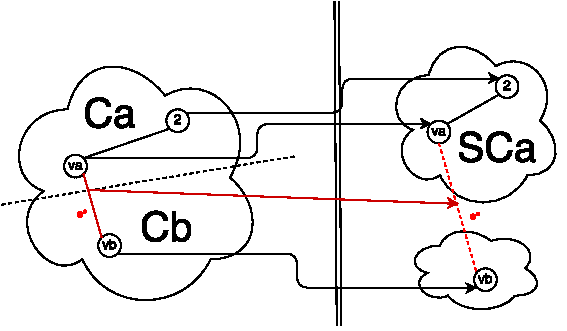
\includegraphics[width=1.4\textwidth,angle=90]{diagrama_ej2.pdf}
   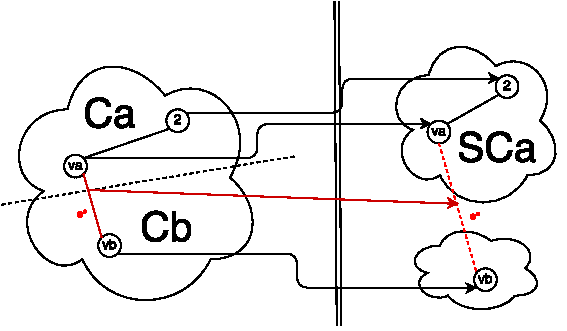
\includegraphics[width=1\textwidth]{diagrama_ej2.pdf}
   \caption{\textbf{Ejemplo gráfico del párrafo anterior}}
   \label{fig:ej2-1}
   \end{center}
\end{figure}

En el gráfico se puede apreciar el fenómeno expuesto en el párrafo anterior,
en donde a modo de ejemplo se están obviando los nodos que no son
imprescindibles a la demostración (se asume que adentro de las ``nubes'' hay
una cantidad indefinida de nodos, y se sabe que dentro de cada ``nube'' los
nodos son conexos).

\end{demostracion}

Dado que todas las soluciones de este problema tienen la misma cantidad de
nodos, ya que son subgrafos generadores de $K_n$, ya que la cantidad de nodos
contenidos en las \violet{$n-(i+1)$} componentes de \violet{$S^{*}$} suma $n$,
y teniendo en cuenta la proposición anterior, se deduce que las
\violet{$n-(i+1)$} componentes de \violet{$S^{*}$} están contenidas en
\redbf{a lo sumo $n-(i+1)$} componentes de \redbf{$S_{n-i}$} o, lo que es lo
mismo, que existe cierto conjunto de \red{\textbf{a lo sumo} $n-(i+1)$ componentes
de $S_{n-i}$ \emph{\textbf{cuyos nodos suman n}}}, y puesto que existen
\redbf{$n-i$} componentes en \redbf{$S_{n-i}$} eso significaría que entre
todas ellas sumarían como mínimo \redbf{$n + [ (n-i) - (n-(i+1)) ] = n+1$} nodos, lo cual es
\textbf{ABSURDO}.

\end{paragraph}

\end{document}

\subsubsection{Cota de complejidad temporal}\label{subsubsec:ej2-cotatemporal}
% ------ headers globales y begin ---------------
\documentclass[11pt, a4paper, twoside]{article}
\usepackage{header_tp2}

\begin{document}{}
% -----------------------------------------------


\end{document}

\subsubsection{Verificación mediante casos de prueba}\label{subsubsec:ej2-casosdeprueba}
% ------ headers globales y begin ---------------
\documentclass[11pt, a4paper, twoside]{article}
\usepackage{header_tp2}

\begin{document}{}
% -----------------------------------------------
A continuación presentamos distintas instancias que sirven para 
verificar que el programa funciona correctamente.

Según la distribución de los pueblos en el mapa, y la relación entre cantidad total de pueblos y la cantidad 
máxima de centrales, podemos separar el conjunto de soluciones en 2 grandes casos: 

\begin{itemize}
	\item Todas las tuberías tienen la misma longitud: 
			\begin{itemize}
				\item Caso \#pueblos $\le$ \#centrales: \\
					En estos casos se coloca en todos los pueblos una central y se va a tener un riesgo mínimo 
					porque no hay tuberías (longitud de tuberías: 0). \\
					
					 \begin{minipage}{0.2\textwidth}
						\begin{tabular}{cc}
						   Input \\
						   \hline
						   3 & 4 \\
						   1 & 1 \\
						   2 & 2 \\
						   3 & 3 \\
						\end{tabular}
					\end{minipage} 
					\begin{minipage}{0.2\textwidth}
						\begin{tabular}{cc}
						   Output \\
						   \hline
						   3 & 0 \\
						   1 &  \\
						   2 &  \\
						   3 &  \\
						\end{tabular}
					\end{minipage} 
					
				\item Caso \#pueblos  $>$ \#centrales: \\
					Todas las tuberías tienen longitud 1 en este ejemplo. \\
					
					\begin{minipage}{0.2\textwidth}
						\begin{tabular}{cc}
						   Input \\
						   \hline
						   6 & 2 \\
						   1 & 1 \\
						   2 & 1 \\
						   1 & 2 \\
						   3 & 3 \\
						   3 & 2 \\
						   4 & 2 \\
						\end{tabular}
					\end{minipage} 
					\begin{minipage}{0.2\textwidth}
						\begin{tabular}{cc}
						   Output \\
						   \hline
						   2 & 4 \\
						   1 &  \\
						   4 &  \\
						   1 & 2 \\
						   3 & 1 \\
						   4 & 5 \\
						   6 & 5 \\
						\end{tabular}
					\end{minipage} 
					
			\end{itemize}
		
	\item Las tuberías tienen longitudes diferentes: 
		    \begin{itemize}
				\item Caso \#pueblos $>$ \#centrales: \\
				   Longitudes de las tuberías: 0, 1, 2. \\
				   \begin{minipage}{0.2\textwidth}
						\begin{tabular}{cc}
							   Input \\
							   \hline
							   6 & 2 \\
							   1 & 1 \\
							   1 & 2 \\
							   2 & 5 \\
							   3 & 1 \\
							   3 & 3 \\
							   4 & 1 \\
						\end{tabular}
					\end{minipage} 
					\begin{minipage}{0.2\textwidth}
						\begin{tabular}{cc}
						   Output \\
						   \hline
						   2 & 4 \\
						   1 &  \\
						   3 &  \\
						   1 & 2 \\
						   4 & 1 \\
						   4 & 6 \\
						   5 & 4 \\
						\end{tabular}
				   \end{minipage}  \\
			
				Misma distribución de los pueblos pero sólo teniendo una central: \\
				Longitudes de las tuberías: 1, 2, $\sqrt[] {5}$. \\
				   \begin{minipage}{0.2\textwidth}
						\begin{tabular}{cc}
						   Input \\
						   \hline
						   6 & 1 \\
						   1 & 1 \\
						   1 & 2 \\
						   2 & 5 \\
						   3 & 1 \\
						   3 & 3 \\
						   4 & 1 \\
						\end{tabular}
				   \end{minipage} 
				   \begin{minipage}{0.2\textwidth}
						\begin{tabular}{cc}
						   Output \\
						   \hline
						   1 & 5 \\
						   1 &   \\
						   1 & 2 \\
						   4 & 1 \\
						   4 & 6 \\
						   5 & 4 \\
						   3 & 5 \\
						\end{tabular}
				   \end{minipage} 
			\end{itemize}
		
\end{itemize}

Ejecutamos el programa con los distintos ejemplos y se llegó a la solución esperada. 
Por lo tanto, podemos concluir que el comportamiento del programa es correcto. 
\end{document}


\subsubsection{Medición empírica de la Performance}\label{subsubsec:ej2-performance}
% ------ headers globales y begin ---------------
\documentclass[11pt, a4paper, twoside]{article}
\usepackage{header_tp2}

\begin{document}{}

Para comprobar que la cota teórica calculada $\bigO{n^2}$ se cumple, decidimos armar un caso aleatorio y 
medir los tiempos de ejecución mientras se variaba $n$ (cantidad total de pueblos del problema). 
Para este caso aleatorio se tomó un valor $k$ (cantidad de centrales) al azar y las coordenadas de los  $n$ 
pueblos también con valores aleatorios. \\
Además, realizamos un gráfico que muestra el cociente $\frac{tiempoDeEjecuci\acute{o}n}{n^2}$ vs $n$ (cantidad
total de pueblos) para confirmar que el algoritmo tiene una complejidad de $\bigO{n^2}$. 
Se tomó nuevamente un caso aleatorio, como el que se mencionó antes, y mientras se variaba el tamaño de entrada $n$, 
medimos los tiempos. Se puede apreciar que a medida que crece $n$ la curva se estabiliza muy cerca de una constante, 
con lo cual concluímos que la cota temporal calculada fue correcta. \\
\clearpage

\begin{figure}[H]
   \begin{center}
   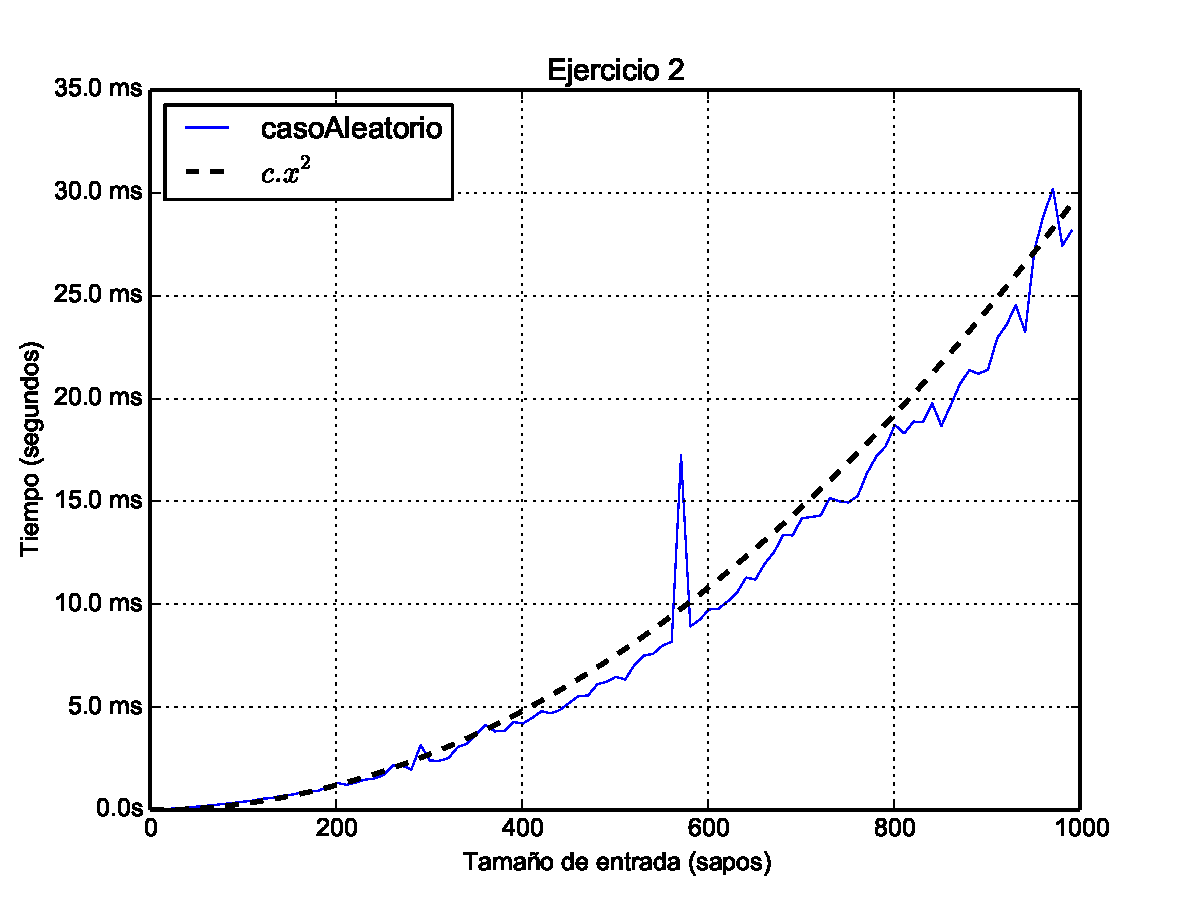
\includegraphics[width=1.4\textwidth, angle=90]{../ej2/graficos/test_tiempoLiso.pdf}
   \caption{\textbf{Muestreo general del Ejercicio 2}}
   \label{fig:ej2-graf-1}
   \end{center}
\end{figure}
\clearpage


\begin{figure}[H]
   \begin{center}
   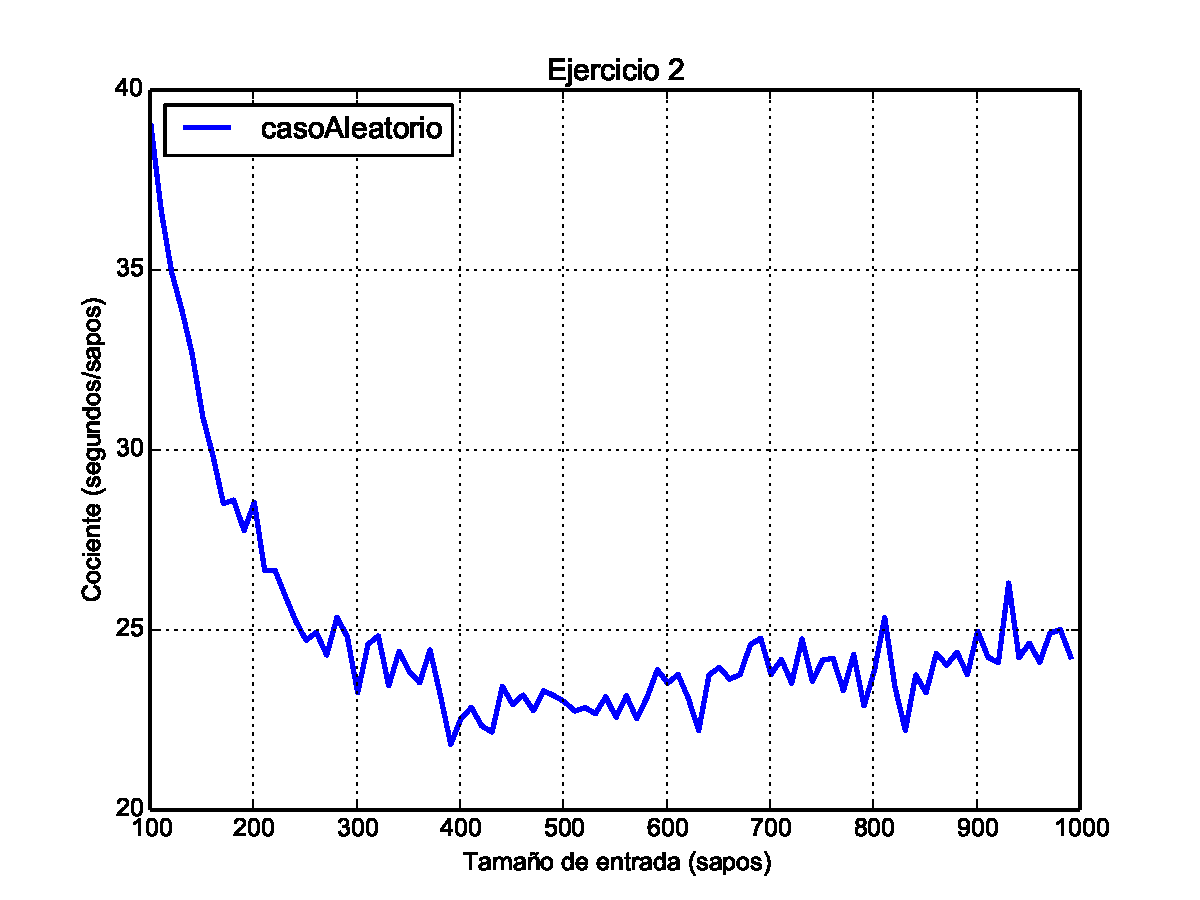
\includegraphics[width=1.4\textwidth,angle=90]{../ej2/graficos/test_Division.pdf}
   \caption{\textbf{Tiempo de ejecución sobre tamaño de la entrada.}}
   \label{fig:ej2-graf-2}
   \end{center}
\end{figure}
\clearpage

Por último, nos pareció interesante realizar una medición de tiempos en función de $k$ (cantidad total de centrales). 
Para este test, las coordenadas de los $n$ pueblos fueron tomadas aleatoriamente, se fijó un $n$ lo 
suficientemente grande, y se midieron los tiempos mientras se variaba el valor de $k$. 
Cuanto mayor sea la cantidad de centrales, la cantidad de conexiones a realizar entre los pueblos es menor, ya que 
como mucho habrá $n - k$ tuberías. Por lo que el tiempo de ejecución del programa disminuiría. 
Si $k = n$ por ejemplo, simplemente se colocaría una central en cada uno de los $n$ pueblos y no haría falta 
ninguna tubería entre ellos.\\
Es evidente, como queda demostrado en la sección de complejidad teórica, que el tiempo de ejecución de nuestro algoritmo es inversamente proporcional a la cantidad de centrales permitidas.
 

% gráfico 3 
\begin{figure}[H]
   \begin{center}
   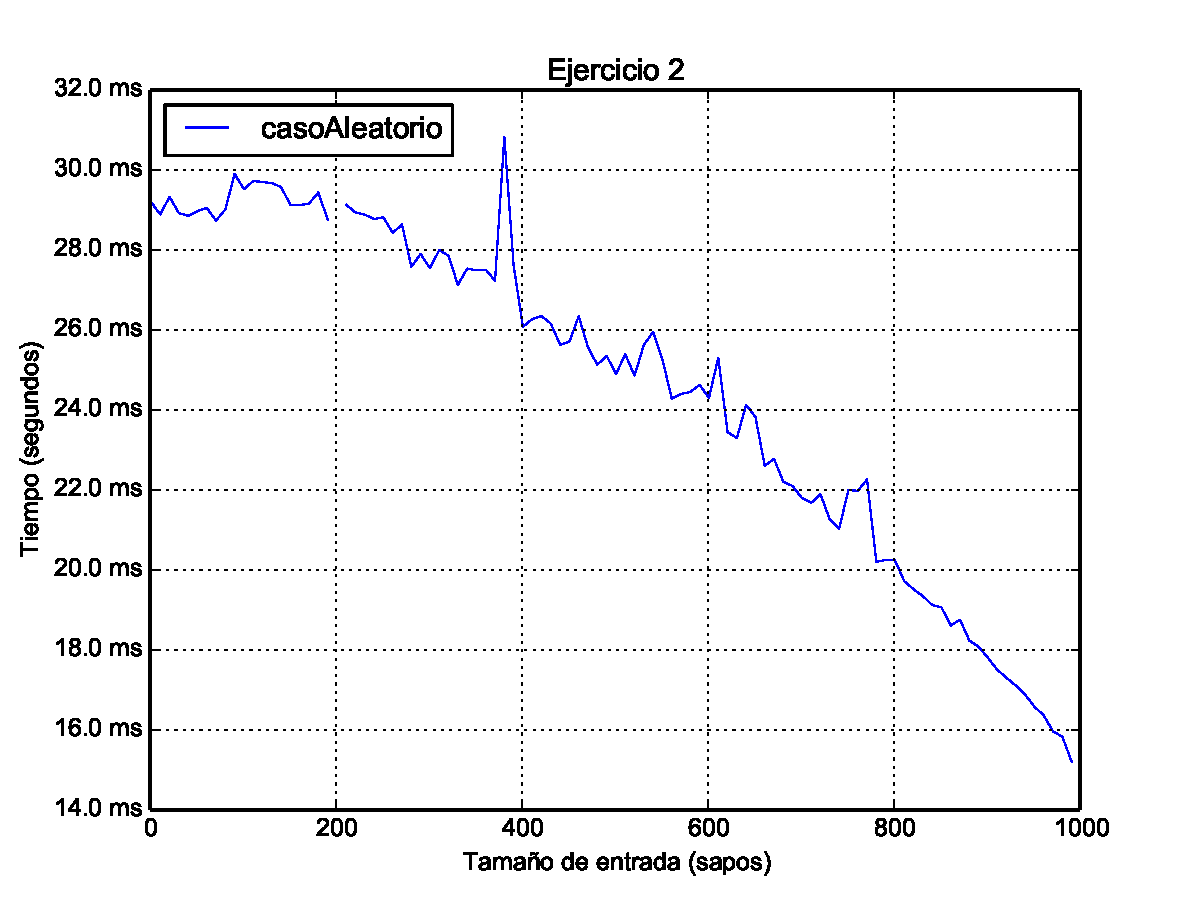
\includegraphics[width=1.4\textwidth,angle=90]{../ej2/graficos/test_variarCantidadCentrales.pdf}
   \caption{\textbf{Tiempo de ejecución en función de la cantidad de centrales ``ITA'' de gas.}}
   \label{fig:ej2-graf-3}
   \end{center}
\end{figure}
\clearpage
   

\end{document}
% -----------------------------------------------


\end{document}

  \newpage
  
  %-- Problema 3 --
  \subsection{Problema 3: Saltos en La Matrix}
  % ------ headers globales y begin ---------------
\documentclass[11pt, a4paper, twoside]{article}
\usepackage{header_tp2}

\begin{document}{}
% -----------------------------------------------

\subsubsection{Descripción}\label{subsubsec:ej3-descripcion}
% ------ headers globales y begin ---------------
\documentclass[11pt, a4paper, twoside]{article}
\usepackage{header_tp2}
\begin{document}{}
% -----------------------------------------------
Se tiene un campo cuadrado de $n \times n$ celdas, cada una de la cuales tiene un resorte propulsor con 
una potencia que va de 1 a $p$. Es decir que es posible ir saltando de una celda cualquier otra mediante estos 
resortes. El juego consiste en que cada participante llegue a la celda $destino$ partiendo 
desde la celda $origen$, realizando la menor cantidad de saltos posibles. Para moverse de una de una celda a otra, 
sólo se permiten movimientos hacia el norte, sur, este u oeste. La potencia que tenga el resorte en una celda, 
es la que limitará la distancia del salto que se puede realizar desde una celda a otra. Además, el participante 
contará con una cantidad $k$ de pontencia extra, la cual podrá utilizar durante el juego, distribuyéndola como le 
sea conveniente en cada salto. Esta potencia extra, le permitirá realizar saltos de mayor distancia. 
La complejidad temporal de peor caso del algoritmo deberá ser de $\bigO{{n^3} \times k}$. \\

\centerbf{Formato de entrada y salida:} 

	\begin{center}
		\begin{minipage}{0.5\textwidth}
			\begin{tabular}{cccccc}
			   & Input \\
			   \hline 
			   n        & $f_{0}$  & $c_{0}$   & $f_{d}$ & $c_{d}$ & k \\
			   $p_{11}$ & $\hdots$ & $p_{1n}$  &&& \\
			   $\vdots$ &          &  $\vdots$ &&& \\
			   $p_{n1}$ &        &  $p_{nn}$   &&& \\
			\end{tabular}
		\end{minipage} 
		\begin{minipage}{0.1\textwidth}
			\begin{tabular}{ccc}
					& Output \\
				   \hline
				   S &   &   \\
				   $f_1$ & $c_1$ & $e_1$ \\
				   $\vdots$ & $\vdots$& $\vdots$\\
				   $f_s$ & $c_s$ & $e_s$ \\
			\end{tabular}
		\end{minipage} 	
	 \end{center} 
	
	\begin{itemize}
		\item n $\#filas$ y $\#columnas$
		\item $(f_{0},c_{0})$ celda $origen$
		\item $(f_{d},c_{d})$ celda $destino$
		\item k $\#unidades$ de potencia extra
		\item $p_{ij}$ potencia máxima del resorte de la celda (i,j), $1 < i,j < n$
		\item S $\#saltos$ de solución óptima
		\item $(f_{i},c_{i})$ celda a la que se realiza el salto, $1 < i < S$
		\item ${e_i}$ $\#unidades$ de potencia extra usados en saldo $i$, $1 < i <S$, $0 < e_i < k$	\\
	\end{itemize} 
 

\begin{ejemplo}\hspace{0em} \\
    \begin{center}
	\begin{minipage}{0.4\textwidth}
			\begin{tabular}{cccccc}
			 & Input \\
			   \hline
			   3 & 1 & 1 & 2 & 3 & 2\\
			   1 & 1 & 1 &   &   &  \\
			   1 & 2 & 1 &   &   &  \\
			   1 & 1 & 1 &   &   &  \\
			\end{tabular}
	\end{minipage}
	\end{center}
	
La siguientes son algunas soluciones posibles (las 2 primeras serían las óptimas): \\	

 \begin{center}
	\begin{minipage}{0.3\textwidth}
			\begin{tabular}{ccc}
				   & Output\\
				   \hline
				   2 &   &   \\
				   2 & 1 & 0 \\
				   2 & 3 & 1 \\
				   \\
				   \\
			\end{tabular}
	\end{minipage} 	
	\begin{minipage}{0.3\textwidth}
			\begin{tabular}{ccc}
				   & Output\\
				   \hline
				   2 &   &   \\
				   1 & 3 & 1 \\
				   2 & 3 & 0 \\
				   \\
				   \\
			\end{tabular}
	\end{minipage} 	\\
	\begin{minipage}{0.3\textwidth}
			\begin{tabular}{ccc}
				   & Output\\
				   \hline
				   3 &   &   \\
				   1 & 2 & 0 \\
				   1 & 3 & 0 \\
				   2 & 3 & 0 \\
				   \\
			\end{tabular}
	\end{minipage} 	
	\begin{minipage}{0.3\textwidth}
			\begin{tabular}{ccc}
				   & Output\\
				   \hline
				   3 &   &   \\
				   3 & 1 & 1 \\
				   3 & 3 & 1 \\
				   2 & 3 & 0 \\
				   \\
			\end{tabular}
	\end{minipage} 	
	\begin{minipage}{0.3\textwidth}
			\begin{tabular}{ccc}
				   & Output\\
				   \hline
				   4 &   &   \\
				   2 & 1 & 0 \\
				   3 & 1 & 0 \\
				   3 & 3 & 1 \\
				   2 & 3 & 0 \\
			\end{tabular}
	\end{minipage} 	
\end{center}	

\end{ejemplo}
 
\end{document}

\subsubsection{Planteamiento de resolución}\label{subsubsec:ej3-resolucion}
% ------ headers globales y begin ---------------
\documentclass[11pt, a4paper, twoside]{article}
\usepackage{header_tp2}

\begin{document}{}
% -----------------------------------------------
% Para una mayor claridad, vamos a describir nuestro algoritmo reduciendo el problema a encontrar la distancia hasta la casilla destino.\\
% Encontrar la secuencia de saltos es algo secundario y está detallado en el código fuente.
% Vamos a pensar el problema como un grafo, siendo cada nodo una posición del tablero con una cantidad de unidades de potencia extra \\
% restantes. Los adyacentes a cada nodo son las casillas (y las unidades extra que quedan para cada caso) a las que puedo llegar usando \\
% mi resorte y mis unidades extra. Se implementó un Breadth-first search. Recorremos primero los nodos a distancia 0, luego a distancia 1, y \\
% así sucesivamente.
% Para cada nodo vamos guardando su distancia desde la posicion de origen. \\
% Inicializamos la distancia hasta la posicion de origen, contando con k unidades extra de potencia, con 0, y el resto de las distancias en INF.\\
% Para cada nodo 'v' que recorremos, sabemos que podemos llegar a sus adyacentes saltando hasta v en v.distancia pasos, y luego saltando al \\
% adyacente 'a' en un paso mas. Luego, podemos decir que a.distancia <= v.distancia + 1. Si no habia recorrido a previamente, \\
% v.distancia + 1 refleja la distancia del camino más corto hasta a. Si ya habia recorrido 'a', su distancia ya está calculada y es menor o \\
% o igual a la de v.\\
% En algun momento llegamos a la casilla destino, ya que el grafo es conexo, y podemos devolver su distancia.
% \nota{Esto de que es conexo, es decir, que cualquier casillero podes llegar a cualquier otro, se puede mencionar en la descripcion del
% problema}


% Pseudocódigo:

% for i=1..n, j=1..n, l=0..k :
%     distancia desde el casillero[i][j], sobrando l unidades extra de potencia = infinito

% distancia hasta el casillero origen, sobrando k unidades extra de potencia = 0

% cola<(int, int, int)> colaBFS

% colaBFS.push(origen, k)

% while ! colaBFS.empty():
%     actual = colaBFS.pop()
%     para cada casillero (x, y) al que puedo llegar desde actual
%         l = unidades extra que quedan tras ir a (x, y)
%         // si no recorri ya ese casillero, quedando esas unidades extra
%         if distancia al casillero (x, y), quedando l unidades extra es menor a infinito :
%             la pongo en 'distancia desde actual' + 1
%             if (es el casillero de destino) break
%             colaBFS.push((x,y), unidades extra que quedan)

% return distancia al destino
\end{document}


\subsubsection{Justificación formal de correctitud}\label{subsubsec:ej3-correctitud}
% ------ headers globales y begin ---------------
\documentclass[11pt, a4paper, twoside]{article}
\usepackage{header_tp2}

\begin{document}{}
% -----------------------------------------------


\end{document}

\subsubsection{Cota de complejidad temporal}\label{subsubsec:ej3-cotatemporal}
% ------ headers globales y begin ---------------
\documentclass[11pt, a4paper, twoside]{article}
\usepackage{header_tp2}

\begin{document}{}
% -----------------------------------------------

% Inicializar las distancias lleva O(n^2 * k)\\
% En el ciclo while recorremos a lo sumo n^2 * k nodos, ya que no recorremos dos veces el mismo nodo.\\
% Para cada nodo miramos todos sus adyacentes, que son a lo sumo todas las casillas en la misma fila, o todas las casillas en la misma\\
% columna, cada casilla con una cantidad de unidades de potencia extra única. En peor caso miramos 2*n nodos, es decir O(n) nodos.\\
% Luego la complejidad del ciclo es O(n^2 * k) * O(n) = O(n^3 * k).\\



\end{document}


\subsubsection{Verificación mediante casos de prueba}\label{subsubsec:ej3-casosdeprueba}
% ------ headers globales y begin ---------------
\documentclass[11pt, a4paper, twoside]{article}
\usepackage{header_tp2}

\begin{document}{}
% -----------------------------------------------
A continuación presentamos distintas instancias que sirven para verificar que el programa funciona correctamente.\\

\begin{itemize}
\item Caso celda origen = celda destino \\
	 \begin{minipage}{0.4\textwidth}
		\begin{tabular}{cccccc}
		   Input \\
		   \hline
		   2 & 1 & 1& 1 & 1 & 0\\
		   1 & 1 &  &   &   &  \\
		   1 & 1 &  &   &   &  \\
		\end{tabular}
	\end{minipage} 
		\begin{minipage}{0.2\textwidth}
			\begin{tabular}{c}
			   Output \\
			   \hline
			   0 \\
				 \\
				 \\
		\end{tabular}
	\end{minipage} 

\item Caso celda origen $\ne$ celda destino 
	\begin{itemize}
		\item Potencia extra = 0 \\
			\begin{itemize}
				\item Potencia máxima del resorte igual para todas las celdas: \\
				\\
					\begin{minipage}{0.4\textwidth}
							\begin{tabular}{cccccc}
							 & Input \\
							   \hline
							   3 & 1 & 1 & 3 & 3 & 0\\
							   1 & 1 & 1 &   &   &  \\
							   1 & 1 & 1 &   &   &  \\
							   1 & 1 & 1 &   &   &  \\
							   \\
							\end{tabular}
						\end{minipage} 
							\begin{minipage}{0.3\textwidth}
								\begin{tabular}{ccc}
								  & Output \\
								   \hline
								   4 &   &   \\
								   2 & 1 & 0 \\
								   3 & 1 & 0 \\
								   3 & 2 & 0 \\
								   3 & 3 & 0 \\
							\end{tabular}
					\end{minipage} 	\\
					\\ \\
					\begin{minipage}{0.4\textwidth}
							\begin{tabular}{cccccc}
							   & Input  \\
							   \hline
							   3 & 1 & 1 & 3 & 3 & 0\\
							   5 & 5 & 5 &   &   &  \\
							   5 & 5 & 5 &   &   &  \\
							   5 & 5 & 5 &   &   &  \\
							\end{tabular}
					\end{minipage} 
					\begin{minipage}{0.3\textwidth}
							\begin{tabular}{ccc}
								   & Output \\
								   \hline
								   2 &   &   \\
								   3 & 1 & 0 \\
								   3 & 3 & 0 \\
								   \\
							\end{tabular}
					\end{minipage} 	\\

				\item Potencia máxima del resorte distinta para las celdas: \\
				\\
				    \begin{minipage}{0.4\textwidth}
							\begin{tabular}{cccccc}
							 & Input \\
							   \hline
							   3 & 1 & 1 & 3 & 3 & 0\\
							   1 & 1 & 2 &   &   &  \\
							   1 & 3 & 1 &   &   &  \\
							   1 & 1 & 1 &   &   &  \\
							   \\
							\end{tabular}
						\end{minipage} 
							\begin{minipage}{0.3\textwidth}
								\begin{tabular}{ccc}
								  & Output \\
								   \hline
								   3 &   &   \\
								   1 & 2 & 0 \\
								   1 & 3 & 0 \\
								   3 & 3 & 0 \\
								    \\
							\end{tabular}
					\end{minipage} 	\\
					\\
					
					\begin{minipage}{0.4\textwidth}
							\begin{tabular}{cccccc}
							 & Input \\
							   \hline
							   4 & 1 & 1 & 4 & 4 & 0\\
							   1 & 1 & 3 & 1 &   &  \\
							   3 & 1 & 1 & 2 &   &  \\
							   1 & 1 & 1 & 1 &   &  \\
							   2 & 1 & 1 & 1 &   &  \\
							\end{tabular}
						\end{minipage} 
							\begin{minipage}{0.3\textwidth}
								\begin{tabular}{ccc}
								  & Output \\
								   \hline
								   3 &   &   \\
								   2 & 1 & 0 \\
								   2 & 4 & 0 \\
								   4 & 4 & 0 \\
								    \\
							\end{tabular}
					\end{minipage} 	\\
			\end{itemize} 
		\item Potencia extra $\ne$ 0 \\
			\begin{itemize}
				\item Potencia máxima del resorte igual para todas las celdas:\\
				\\
					\begin{minipage}{0.4\textwidth}
							\begin{tabular}{cccccc}
							 & Input \\
							   \hline
							   3 & 1 & 1 & 3 & 3 & 5\\
							   1 & 1 & 1 &   &   &  \\
							   1 & 1 & 1 &   &   &  \\
							   1 & 1 & 1 &   &   &  \\
							\end{tabular}
						\end{minipage} 
						\begin{minipage}{0.3\textwidth}
							\begin{tabular}{ccc}
								   & Output \\
								   \hline
								   2 &   &   \\
								   3 & 1 & 1 \\
								   3 & 3 & 1 \\
								   \\
							\end{tabular}
					    \end{minipage} 	\\
				\item Potencia máxima del resorte distinta para las celdas: \\
				\\
					\begin{minipage}{0.4\textwidth}
								\begin{tabular}{cccccc}
								 & Input \\
								   \hline
								   3 & 1 & 1 & 3 & 3 & 1\\
								   1 & 1 & 2 &   &   &  \\
								   1 & 3 & 1 &   &   &  \\
								   1 & 1 & 1 &   &   &  \\
								\end{tabular}
							\end{minipage} 
								\begin{minipage}{0.3\textwidth}
									\begin{tabular}{ccc}
									  & Output \\
									   \hline
									   2 &   &   \\
									   1 & 3 & 1 \\
									   3 & 3 & 0 \\
									   \\
								\end{tabular}
					\end{minipage} \\
					\\
					
					\begin{minipage}{0.4\textwidth}
							\begin{tabular}{cccccc}
							 & Input \\
							   \hline
							   4 & 1 & 1 & 4 & 4 & 3\\
							   1 & 1 & 3 & 1 &   &  \\
							   3 & 1 & 1 & 2 &   &  \\
							   1 & 1 & 1 & 1 &   &  \\
							   2 & 1 & 1 & 1 &   &  \\
							\end{tabular}
						\end{minipage} 
							\begin{minipage}{0.3\textwidth}
								\begin{tabular}{ccc}
								  & Output \\
								   \hline
								   2 &   &   \\
								   4 & 1 & 2 \\
								   4 & 4 & 1 \\
								    \\
								    \\
							\end{tabular}
					\end{minipage} 						
				
			\end{itemize}
	\end{itemize}
\end{itemize}

Ejecutamos el programa con los distintos ejemplos y se llegó a la solución esperada. 
Por lo tanto, podemos concluir que el comportamiento del programa es correcto. 

\end{document}


\subsubsection{Medición empírica de la Performance}\label{subsubsec:ej3-performance}
% ------ headers globales y begin ---------------
\documentclass[11pt, a4paper, twoside]{article}
\usepackage{header_tp2}
\begin{document}{}
% -----------------------------------------------
%á

%%%
%%Cosas
%%%


\end{document}
% -----------------------------------------------


\end{document}
\label{subsec:ej3}
  \newpage

%-- Apéndices --
\section{Apéndices}
  
  \subsection{Código Fuente (resumen)}\label{subsec:codigo-fuente}
  % ------ headers globales y begin ---------------
\documentclass[11pt, a4paper, twoside]{article}
\usepackage{header_tp2}
\begin{document}{}
% -----------------------------------------------
%á

% -----------------------------------------------
\end{document}
  \clearpage
  
  %
  % - Para la reentrega -
  %
  %\subsection{Informe de Modificaciones}
  %% ------ headers globales y begin ---------------
\documentclass[11pt, a4paper, twoside]{article}
\usepackage{header_tp2}
\begin{document}{}
% -----------------------------------------------
%á


% -----------------------------------------------
\end{document}
  %\clearpage
  
  %-- Bibliografia --
  %\subsection{Bibliografía}
  %\begin{thebibliography}{99}
% 
%   \bibitem{lib:brassard} G. Brassard, P. Bratley, \textit{Fundamental of Algorithmics}, Prentice Hall,  1996, Chapter 6.2, \enquote{General characteristics of greedy algoritmhs}, Chapter 9.6, \enquote{Backtracking}, 
%   \bibitem{lib:cormen} Cormen, Leiserson, Rivest \textit{Introduction to Algorithms}, 2001, Chapter 16 \enquote{Greedy Algorithms}.
%   \bibitem{stl:stl} \texttt{http://www.cplusplus.com/reference/stl/}
%   \bibitem{stl:set} \texttt{http://www.cplusplus.com/reference/set/set/}
%   \bibitem{stl:vector} \texttt{http://www.cplusplus.com/reference/vector/vector/}
%   \bibitem{stl:pqueue} \texttt{http://www.cplusplus.com/reference/queue/priority\_queue/}
%   \bibitem{wiki:greedy} \texttt{http://en.wikipedia.org/wiki/Greedy\_algorithm\#Specifics}
%   \bibitem{wiki:back} \texttt{http://en.wikipedia.org/wiki/Backtracking\#Usage\_considerations}

  %\end{thebibliography}

\end{TP2}
\end{document}
